%%-----------------------------------------------------------------------------
%%
%%                                   Sean Mauch
%%                       California Institute of Technology
%%                        @ 1995-2004 No Rights Reserved
%%
%%-----------------------------------------------------------------------------
\documentclass{slides}

% HEADER FILE FOR THE SLIDES


\usepackage{amsmath}
\usepackage{theorem}
% Maybe I can get rid of the following three.
\usepackage{epic}
\usepackage{curves}
\usepackage{eepic}
\usepackage{amssymb}
\usepackage{makeidx}

\usepackage[pdftex]{graphicx}
\pdfcompresslevel=9
\usepackage{color}

%  \pagestyle{plain}
%  \topmargin=-0.75in
%  \headsep=0in
%  \headheight=0in
%  \footskip=.5in
%  \textheight=6in
%  \textwidth=8in
%  \oddsidemargin=-0.75in
%  \evensidemargin=-0.75in
%  \newcommand{\theoremfamily}{\sffamily}


% CONTINUE: FIX
%----------------------------------------------------------------------------
\theoremstyle{plain}
\theoremheaderfont{\theoremfamily\normalsize\bfseries}
\theorembodyfont{\theoremfamily\slshape\normalsize}
\newtheorem{Example}{Example}


\theoremstyle{break}
\theorembodyfont{\theoremfamily\normalsize}
\newtheorem{Exercise}{Exercise}


\theoremstyle{break}
\theorembodyfont{\theoremfamily\normalsize}
\newtheorem{Hint}{Hint}


\theoremstyle{break}
\theorembodyfont{\theoremfamily\normalsize}
\newtheorem{Solution}{Solution}


\theoremstyle{break}
\theorembodyfont{\theoremfamily\normalsize}
\newtheorem{QuizProblem}{Problem}


\theoremstyle{break}
\theorembodyfont{\theoremfamily\normalsize}
\newtheorem{QuizSolution}{Solution}


\theoremstyle{plain}
\theorembodyfont{\theoremfamily\large}
\newtheorem{Theorem}{\large Theorem}


\theoremstyle{plain}
\theorembodyfont{\theoremfamily\large}
\newtheorem{Result}{\large Result}

\setlength{\theorempreskipamount}{12pt}
\setlength{\theorempostskipamount}{12pt}

\newcommand{\resultwidth}{\textwidth}
\newcommand{\resultskip}{\vspace{.1in}}
\newenvironment{ResultBox}{\begin{minipage}{\resultwidth}\begin{Result}}
                                {\end{Result}\end{minipage}}

%-----------------------------------------------------------------------------

\newcommand{\dd}{\mathrm{d}}

\newcommand{\e}{\mathop{\mathrm{e}}\nolimits}
\newcommand{\erf}{\mathop{\mathrm{erf}}\nolimits}
\newcommand{\erfc}{\mathop{\mathrm{erfc}}\nolimits}
\newcommand{\berfc}{\mathop{\mathbf{erfc}}\nolimits}
\newcommand{\bsin}{\mathop{\mathbf{sin}}\nolimits}
\newcommand{\bcos}{\mathop{\mathbf{cos}}\nolimits}
\newcommand{\sign}{\mathop{\mathrm{sign}}\nolimits}
\newcommand{\rank}{\mathop{\mathrm{rank}}\nolimits}
\newcommand{\nullspace}{\mathop{\mathrm{nullspace}}\nolimits}
\newcommand{\thespan}{\mathop{\mathrm{span}}\nolimits}
\newcommand{\Res}{\mathop{\mathrm{Res}}\nolimits}
\newcommand{\Ei}{\mathop{\mathrm{Ei}}\nolimits}
\newcommand{\PV}{\mathop{\mathrm{PV}}\nolimits}
\newcommand{\pvint}{- \negthickspace \negthickspace \negthickspace
                        \negmedspace \int}
\newcommand{\pv}{- \negthickspace \negthickspace \negthickspace \negmedspace}
\newcommand{\textpv}{- \negthickspace \negthickspace \negthickspace}
\newcommand{\Log}{\mathop{\mathrm{Log}}\nolimits}
\newcommand{\Arg}{\mathop{\mathrm{Arg}}\nolimits}
\newcommand{\sech}{\mathop{\mathrm{sech}}\nolimits}
\newcommand{\csch}{\mathop{\mathrm{csch}}\nolimits}
\newcommand{\arcsinh}{\mathop{\mathrm{arcsinh}}\nolimits}
\newcommand{\arccosh}{\mathop{\mathrm{arccosh}}\nolimits}
\newcommand{\arctanh}{\mathop{\mathrm{arctanh}}\nolimits}
\newcommand{\Arcsin}{\mathop{\mathrm{Arcsin}}\nolimits}
\newcommand{\Arccos}{\mathop{\mathrm{Arccos}}\nolimits}
\newcommand{\Arctan}{\mathop{\mathrm{Arctan}}\nolimits}

%% I don't know the package that would define these.
%% Hopefully I can find it and remove these definitions.
\newcommand{\setN}{\mathbb{N}}
\newcommand{\setZ}{\mathbb{Z}}
\newcommand{\setR}{\mathbb{R}}
\newcommand{\setC}{\mathbb{C}}




\begin{document}



%%============================================================================
\begin{slide}
\begin{center}
\begin{Large}
Complex Numbers
\end{Large}
\end{center}


I'm sorry.  You have reached an imaginary number.  Please rotate your phone
$90$ degrees and dial again.

\begin{flushright}
  -Message on answering machine of Cathy Vargas.
\end{flushright}


\end{slide}






%%============================================================================
\begin{slide}
\begin{center}
\begin{large}
Complex Numbers: Shortcomings of real numbers.
\end{large}
\end{center}

When you started algebra, you learned that the quadratic equation:
$x^2 + 2 a x + b = 0$ has either two, one or no solutions.  For example:
\begin{itemize}
\item
  $x^2 - 3 x + 2 = 0$ has the two solutions $x = 1$ and $x = 2$.
\item
  For $x^2 - 2 x + 1 = 0$, $x = 1$ is a solution of multiplicity two.
\item
  $x^2 + 1 = 0$ has no solutions.
\end{itemize}
\end{slide}



%%============================================================================
\begin{slide}
This is a little unsatisfactory.  
We can formally solve the general quadratic equation.
\begin{gather*}
  x^2 + 2 a x + b = 0 
  \\
  (x + a)^2 = a^2 - b 
  \\
  x = -a \pm \sqrt{a^2 - b}
\end{gather*}
However, the solutions are defined only when the discriminant $a^2 -
b$ is non-negative.  This is because the square root function $\sqrt{x}$
is a bijection from $\mathbb{R}^{0+}$ to $\mathbb{R}^{0+}$. 
\begin{center}
  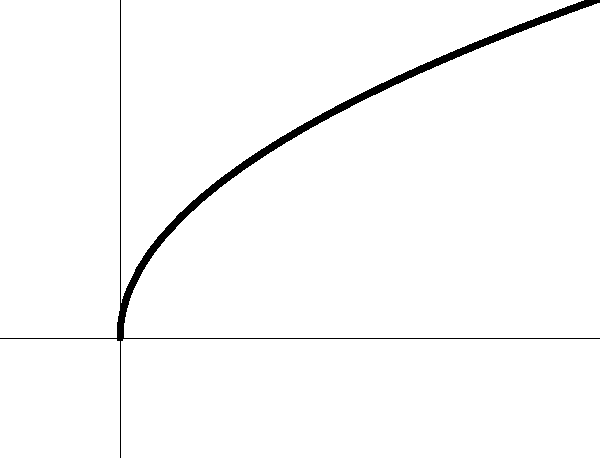
\includegraphics[width=0.3\textwidth]{yesqrtx}
\end{center}
\end{slide}


%%============================================================================
\begin{slide}
\begin{center}
\begin{large}
A new mathematical constant.
\end{large}
\end{center}
We cannot solve $x^2 = -1$ because the square root of $-1$ is not defined.  
We create a new symbolic constant $\sqrt{-1}$.  
We will treat $\sqrt{-1}$ as we would a real constant like $\pi$ or a 
formal variable like $x$, i.e. 
\[ 
\sqrt{-1} + \sqrt{-1} = 2 \sqrt{-1}.
\]
This constant has the property:
\[
\left( \sqrt{-1} \right)^2 = -1.
\]
Now we can express the solutions
of $x^2 = -1$ as $x = \sqrt{-1}$ and $x = - \sqrt{-1}$.  These satisfy
the equation since 
\[
\left( \sqrt{-1} \right)^2 = -1
\]
and 
\[
\left( - \sqrt{-1} \right)^2 = (-1)^2 \left( \sqrt{-1} \right)^2 = -1.
\]
Note that we can express the square root of any negative real number in 
terms of $\sqrt{-1}$: 
\[
\sqrt{-r} = \sqrt{-1} \sqrt{r}\ \mathrm{for}\ r \geq 0.  
\]
\end{slide}



%%============================================================================
\begin{slide}
\begin{center}
\begin{large}
Euler's notation.
\end{large}
\end{center}
Euler introduced the notation of using the letter $i$ to denote $\sqrt{-1}$.
We will use the symbol $\imath$, an $i$ without a dot, to denote 
$\sqrt{-1}$.%
\footnote{
  Electrical engineering types prefer to use $\jmath$ or $j$ to denote
  $\sqrt{-1}$.
  }

We call any number of the form $\imath b$, 
$b \in \mathbb{R}$, a \textit{pure imaginary number}.%
\footnote{
  ``Imaginary'' is an unfortunate term.  Real numbers are 
  artificial; constructs of the mind.  Real numbers are no more real than
  imaginary numbers.
  }

Let $a$ and $b$ be real numbers.  The product of a real number and an 
imaginary number is an imaginary number: $(a)(\imath b) = \imath (a b)$.
The product of two imaginary numbers is a real number: 
$(\imath a)(\imath b) = - a b$.  However the sum of a real number and an 
imaginary number $a + \imath b$ is neither real nor imaginary.
We call numbers of the form $a + \imath b$ \textit{complex numbers}.%
\footnote{
  Here complex means ``composed of two or more parts'', not
  ``hard to separate, analyze, or solve''.  Those who disagree have a 
  complex number complex.
  }
\end{slide}


\end{document}

